% !TEX TS-program = lualatex
% !TEX encoding = UTF-8 Unicode
\documentclass{article}
\usepackage{lmodern}
\usepackage{graphicx}
\graphicspath{{doc/assets/}{../doc/assets/}{assets/}{../assets/}{../}}

\usepackage[
  paperwidth=338mm, paperheight=190mm,
  top=0mm, bottom=0mm, left=0mm, right=0mm
]{geometry}

% -- ROBUST FONT FIX FOR LUALATEX & OVERLEAF --
\usepackage{fontspec}
\IfFontExistsTF{Roboto}{
  \setsansfont{Roboto}
}{
  \IfFontExistsTF{Arial}{
    \setsansfont{Arial}[
      ItalicFont={Arial},
      ItalicFeatures={FakeSlant=0.25},
      BoldFont={Arial Bold},
      BoldItalicFont={Arial Bold},
      BoldItalicFeatures={FakeSlant=0.25}
    ]
  }{
    \IfFontExistsTF{Noto Sans}{
      \setsansfont{Noto Sans}
    }{
      \IfFontExistsTF{Liberation Sans}{
        \setsansfont{Liberation Sans}
      }{
        \IfFontExistsTF{TeX Gyre Heros}{
          \setsansfont{TeX Gyre Heros}
        }{
          % Fallback mặc định
        }
      }
    }
  }
}
\renewcommand{\familydefault}{\sfdefault}
% ---------------------------------------------

\usepackage{xcolor}
\usepackage{tikz}
\usepackage{fontawesome5}
\usepackage{pgfplots}
\pgfplotsset{compat=1.18}
\usetikzlibrary{calc, matrix, arrows.meta, shapes.geometric}
\usepackage[hidelinks]{hyperref}
\pagestyle{empty}
\parindent=0pt

\newcommand{\TOCitem}[1]{{\color{sap}\vrule width 2pt height 8pt depth 0pt}\ #1}

%── Bảng màu chuẩn hóa thanh lịch (Pure Blue/Yellow)
\definecolor{sap}{HTML}{0000FF}           % Primary: Xanh lam thuần
\definecolor{cyel}{HTML}{FFFF00}         % Secondary: Vàng thuần
\definecolor{cslate}{HTML}{64748B}
\definecolor{cneg}{HTML}{D32F2F}
\definecolor{cpos}{HTML}{2E7D32}
\definecolor{cgry}{HTML}{757575}
\definecolor{clightgray}{HTML}{F8F9FA}

% Màu nền khối Insight Box
\definecolor{cgr}{HTML}{2E7D32}
\definecolor{cbl}{HTML}{1565C0}
\definecolor{cbk}{HTML}{424242}
\colorlet{bggr}{cgr!8}
\colorlet{bgbl}{cbl!8}
\colorlet{bgbk}{cbk!8}

%── Định hình cấu trúc pgfplots hóa biểu đồ
\pgfplotsset{
  empty legend/.style={draw=none, fill=none},
  dashmod/.style={dashed, line width=2.5pt, mark=none},
  solproj/.style={solid,  line width=2.5pt, mark=none},
  hlchart/.style={
    clip=false,
    scale only axis=true,
    xmin=0.5, xmax=7.5, ymin=0, ymax=5.9,
    xtick={1,2,3,4,5,6,7},
    xticklabels={W1,W2,W3,{W4$^\star$},W5,W6,W7},
    x tick label style={font=\fontsize{15}{18}\selectfont, text=cgry!80!black},
    y tick label style={font=\fontsize{15}{18}\selectfont, text=cgry!80!black},
    ylabel={},
    xlabel={},
    grid=both,
    minor ytick={0,0.5,...,5.5},
    minor grid style={gray!8,  line width=0.15pt},
    major grid style={gray!18, line width=0.30pt},
    axis line style={gray!35,  line width=0.40pt},
    tick style={gray!35, line width=0.40pt},
    legend style={
      at={(0.5, -0.12)},
      anchor=north,
      font=\fontsize{14}{17}\selectfont,
      draw=none, fill=none,
      legend columns=4,
      column sep=4ex,
      row sep=1ex
    },
    legend cell align=left,
  }
}

%── Hệ thống các Macros tạo khối giao diện nhanh
\newcommand{\Card}[7]{%
  \begin{scope}[shift={(#1mm,#2mm)}]
    \fill[clightgray,rounded corners=4pt] (0,0) rectangle (50mm,32mm);
    \node[anchor=north west, font=\fontsize{11}{13}\selectfont\color{cslate}, text width=42mm] at (4mm, 28mm) {\MakeUppercase{#3}};
    \node[anchor=north west, font=\fontsize{28}{32}\selectfont\bfseries\color{sap}] at (4mm, 23mm) {#4};
    \node[anchor=north west, font=\fontsize{12}{14}\selectfont\color{#7}] at (4mm, 9mm) {#6 \textcolor{cslate!75}{(D.Án: #5)}};
  \end{scope}
}

\newcommand{\Insight}[9]{%
  \begin{scope}[shift={(#1mm,#2mm)}]
    \fill[#3,rounded corners=4pt] (0,0) rectangle (98mm,50mm);
    \node[anchor=north west, font=\fontsize{22}{26}\selectfont\color{#4}] at (4mm, 46mm) {#5};
    \node[anchor=north west, text width=92mm, align=left] at (4mm, 37mm) {
        \fontsize{10.5}{13.5}\selectfont\color{#4!35!black}
        \textbullet\ \ #6 \par \textbullet\ \ #7 \par \textbullet\ \ #8 \par \vspace{3.5pt}
        \textcolor{#4}{\faHandPointRight}\ \ \textbf{#9}
    };
  \end{scope}
}

\newcommand{\TitleLine}[1]{%
  \draw[cyel, line width=6pt] (17mm, -10mm) -- (17mm, -25mm);
  \node[anchor=west, font=\fontsize{35}{40}\selectfont\bfseries, text=sap] at (21mm, -17.5mm) {#1};
}

\newcommand{\ContentBox}[4]{%
  \begin{scope}[shift={(#1mm,#2mm)}]
    \fill[clightgray, rounded corners=4pt] (0,0) rectangle (95mm,42mm);
    \node[anchor=north west, font=\fontsize{16}{20}\selectfont\bfseries\color{sap}, text width=85mm] at (5mm, 37mm) {#3};
    \node[anchor=north west, font=\fontsize{12}{16}\selectfont\color{cbk}, text width=85mm] at (5mm, 22mm) {#4};
  \end{scope}
}

\newcommand{\vtwomark}{%
  \addplot[black!22,solid,line width=1.5pt,mark=none,forget plot] coordinates{(3.5,0)(3.5,5.9)};
  \node[font=\fontsize{15}{18}\selectfont,text=black!38,anchor=south west] at (axis cs:3.55,5.4) {V2$\to$};
}

\begin{document}

% ===================================================================
% SLIDE 4: Phân hệ cấu hình - Tổng quát (Kế thừa dữ liệu sơ đồ từ PDF Trang 3)
% ===================================================================
\begin{tikzpicture}[remember picture, overlay]
  \coordinate (NW) at (current page.north west);
  \begin{scope}[shift={(NW)}]
    \TitleLine{Phân hệ cấu hình - Tổng quát}

    \ContentBox{17}{-65}{Trung tâm Điều phối Cấu hình}{Chủ sở hữu cơ sở dữ liệu SQLite và kiểm soát toàn bộ tham số cấu hình.}
    \ContentBox{17}{-108}{Quản lý Phiên \& Luồng Chơi}{Xử lý chuyển đổi trạng thái Menu, Cốt truyện và Lõi qua router thông minh.}
    \ContentBox{17}{-151}{Bảng Xếp hạng Toàn cầu}{Tích hợp thuật toán sắp xếp và đồng bộ dữ liệu với Cloudflare D1.}

    % Khối sơ đồ Usecase cấu hình tái lập trung thực theo sơ đồ trang 3 PDF gốc
    \begin{scope}[shift={(165mm, -55mm)}, scale=1.35, every node/.append style={transform shape}]
        \draw[cslate, thick, rounded corners=4pt] (0,0) rectangle (7.5,-5.5);
        \node[anchor=north, font=\fontsize{12}{14}\selectfont\bfseries\color{sap}] at (3.75, -0.2) {Sơ đồ usecase (Cấu hình)};
        
        \node[circle, draw=cslate, fill=clightgray, minimum size=0.8cm] (p) at (-1.6, -2.7) {};
        \node[below=2pt, font=\fontsize{11}{13}\selectfont\color{cbk}] at (p.south) {Người chơi};
        
        \node[circle, draw=sap, fill=clightgray, minimum size=0.8cm] (net) at (9.1, -2.7) {};
        \node[below=2pt, font=\fontsize{11}{13}\selectfont\color{cbk}] at (net.south) {Cloudflare D1};
        
        \begin{scope}[every node/.style={ellipse, draw=cslate, fill=white, minimum width=3.5cm, inner sep=2pt, font=\fontsize{9}{11}\selectfont\color{cbk}}]
            \node (u1) at (3.75,-1.1) {Tùy chỉnh hệ thống};
            \node (u2) at (3.75,-2.0) {Chọn nhánh cốt truyện};
            \node (u3) at (3.75,-2.9) {Tra cứu xếp hạng};
            \node (u4) at (3.75,-3.8) {Điều phối luồng chơi};
            \node (u5) [draw=sap, font=\fontsize{9}{11}\selectfont\bfseries\color{sap}] at (3.75,-4.7) {Đồng bộ Dữ liệu};
        \end{scope}

        \foreach \i in {1,2,3,4} \draw[->, thick, draw=cslate] (p) -- (u\i.west);
        \draw[->, thick, draw=sap] (net) -- (u5.east);
        \draw[->, thick, dashed, draw=sap] (u5.north) to[bend right=30] (u3.east);
    \end{scope}

    \node[anchor=north west, text width=290mm, font=\fontsize{13}{17}\selectfont\color{cbk}] at (17mm, -156mm) {
        \textbf{Đặc điểm cốt lõi:} Đóng vai trò là trung tâm não bộ của hệ thống.
        Quản lý bền vững trạng thái cài đặt và tiến trình người chơi thông qua SQLite ngoại tuyến, đồng thời tích hợp thuật toán sắp xếp thông minh và đồng bộ hóa thành tích với nền tảng Cloudflare D1.
    };
  \end{scope}
\end{tikzpicture}
\newpage

% ===================================================================
% SLIDE 5: Phân hệ cấu hình - V1 vs V2
% ===================================================================
\begin{tikzpicture}[remember picture, overlay]
  \coordinate (NW) at (current page.north west);
  \begin{scope}[shift={(NW)}]
    \TitleLine{Phân hệ cấu hình - V1 vs V2}
    \node[anchor=north west, label={[sap]below:V1}] at (17mm, -35mm) {
      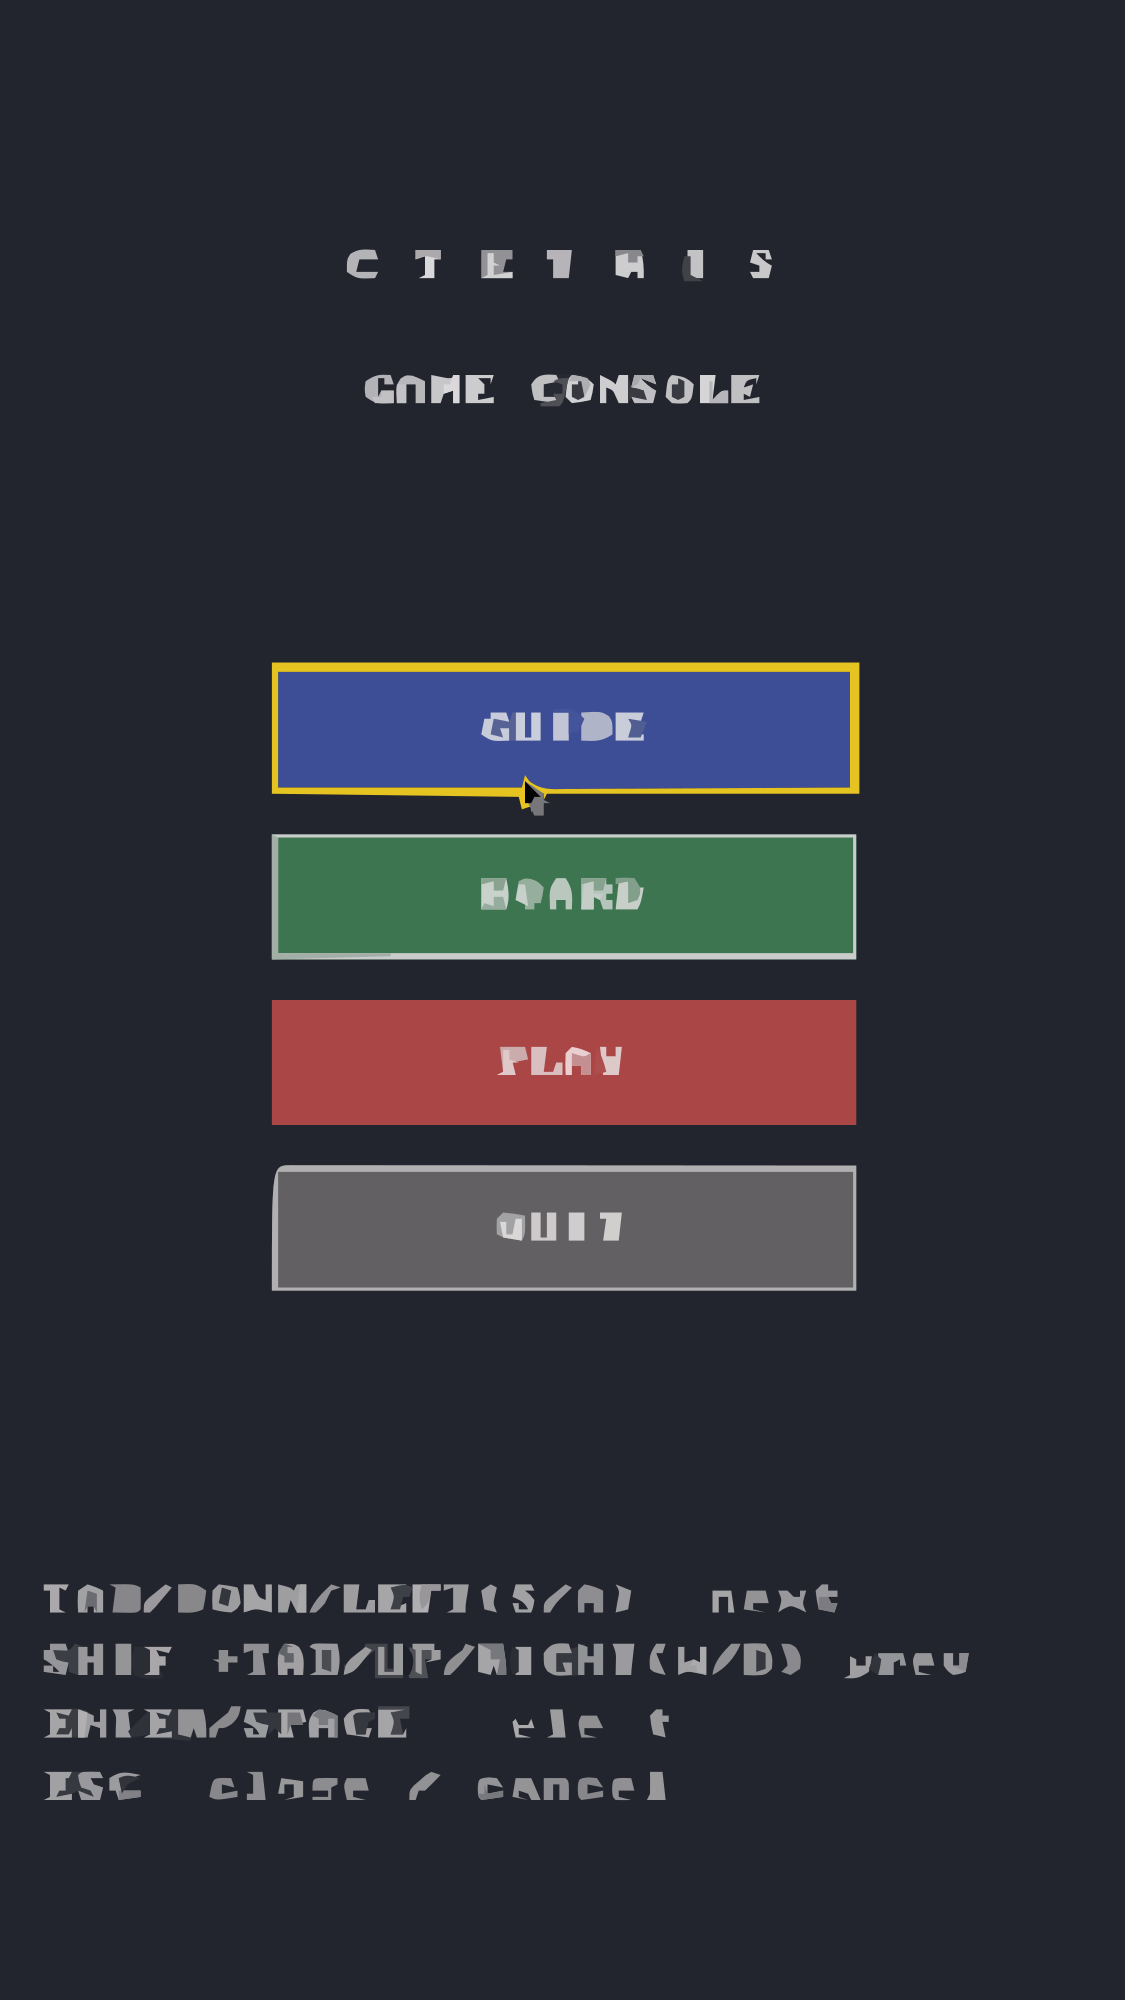
\includegraphics[width=95mm, height=135mm, keepaspectratio]{09-gameConsoleGuide-screenshot.png}
    };
    \draw[red, dashed, line width=2.5pt] (122mm, -35mm) -- (122mm, -170mm);
    \node[anchor=north west, label={[sap]below:V2 - Menu}] at (132mm, -35mm) {
      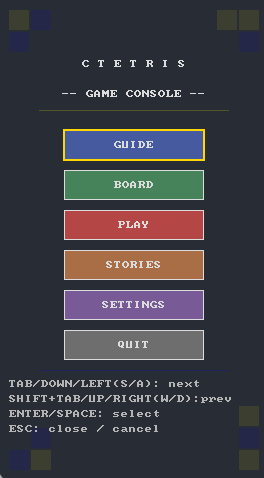
\includegraphics[width=95mm, height=135mm, keepaspectratio]{09-gameConsoleGuide-screenshot-v2.png}
    };
    \node[anchor=north west, label={[sap]below:V2 - Stories}] at (232mm, -35mm) {
      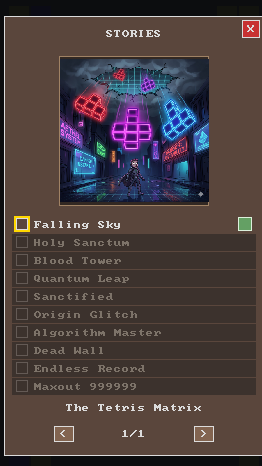
\includegraphics[width=95mm, height=135mm, keepaspectratio]{09-gameConsoleGuide-screenshot-v2-stories.png}
    };
  \end{scope}
\end{tikzpicture}
\newpage

% ===================================================================
% SLIDE 6: Phân hệ cấu hình - Thống kê (Áp dụng khung lưới trục từ PDF Trang 5)
% ===================================================================
\begin{tikzpicture}[remember picture, overlay]
  \coordinate (NW) at (current page.north west);
  \begin{scope}[shift={(NW)}]
      \TitleLine{Phân hệ cấu hình - Thống kê}
      \Card{17}{-58}{Tổng Tin Nhắn}{68.4}{206.3}{$\downarrow$\,17.6\,\%}{cpos}
      \Card{71}{-58}{Tin Nhắn (Người)}{57.3}{172.8}{$\downarrow$\,20.0\,\%}{cpos}
      \Card{17}{-94}{Task Hoàn Thành}{20.9}{61.7}{$\downarrow$\,10.5\,\%}{cpos}
      \Card{71}{-94}{Lỗi Phát Sinh}{16.7}{47.9}{$\uparrow$\,30.5\,\%}{cneg}
      \Card{17}{-130}{Tổng Commits}{58.5}{163.5}{$\downarrow$\,15.2\,\%}{cpos}
      \Card{71}{-130}{Xung Đột}{15.8}{47.4}{$\uparrow$\,3.6\,\%}{cneg}
      
      % Hệ thống biểu đồ lưới nẹp trục số liệu hoàn chỉnh cho phân hệ gameConsole
      \begin{axis}[at={(127mm,-106mm)},anchor=south west, width=194mm,height=80mm,hlchart]
        \vtwomark
        \addlegendimage{empty legend}\addlegendentry{\textbf{Phân hệ}}
        \addplot[cgr,dashmod] coordinates{(1,.88)(2,.88)(3,.88)(4,.78)(5,.78)(6,.78)(7,.62)}; \addlegendentry{human/bot}
        \addplot[cbl,dashmod] coordinates{(1,.27)(2,.27)(3,.27)(4,2.91)(5,1.98)(6,1.98)(7,1.83)}; \addlegendentry{issue/task}
        \addplot[cbk,dashmod] coordinates{(1,.19)(2,.19)(3,.19)(4,.61)(5,.27)(6,.27)(7,.49)}; \addlegendentry{conflict/commit}
        \addlegendimage{empty legend}\addlegendentry{\textbf{Dự án}}
        \addplot[cgr,solproj] coordinates{(1,.88)(2,.88)(3,.88)(4,.78)(5,.78)(6,.78)(7,.62)}; \addlegendentry{human/bot}
        \addplot[cbl,solproj] coordinates{(1,.32)(2,.32)(3,.32)(4,3.60)(5,2.10)(6,2.10)(7,1.49)}; \addlegendentry{issue/task}
        \addplot[cbk,solproj] coordinates{(1,.20)(2,.20)(3,.20)(4,.66)(5,.29)(6,.29)(7,.49)}; \addlegendentry{conflict/commit}
      \end{axis}
      
      \Insight{17}{-184}{bggr}{cgr}{\faSlack}{Sp1 (W1-2): Tỷ lệ giao tiếp ổn định 0.88.}{Sp2 (W3-4): Giảm 0.78 khi tích hợp DB.}{Sp3 (W5-7): Cán mốc 0.62 – cấu hình vững.}{Tương tự các phân hệ khác, tỷ lệ giao tiếp cao ở thời gian đầu và giảm dân khi đã nắm vũng công nghệ.}
      \Insight{120}{-184}{bgbl}{cbl}{\faTrello}{Sp1 (W1-2): Lỗi thấp nhất cả dự án (0.27).}{Sp2 (W3-4): Vọt lên 2.91 – tích hợp Cloudflare D1.}{Sp3 (W5-7): Chưa về chuẩn, duy trì 1.83.}{Đây là phân hệ có tỷ lệ phát sinh lỗi cao nhất và ngày càng gia tăng, nghĩa là càng làm nhiều, càng nhiều lỗi.}
      \Insight{223}{-184}{bgbk}{cbk}{\faGithub}{Sp1 (W1-2): Xung đột rất thấp (0.19).}{Sp2 (W3-4): Tăng lên 0.61 khi merge schema DB.}{Sp3 (W5-7): Kiểm soát còn 0.49 sau chia nhánh.}{Các xung đột xảy ra chủ yếu khi tích hợp, và vẫn còn xuất hiện khi chia nhánh, cho thấy cần cải thiện quy trình làm việc nhóm.}
  \end{scope}
\end{tikzpicture}
\newpage

\end{document}